% This document must be compiled with LuaLaTeX
\documentclass[12pt,article]{memoir}

\usepackage[letterpaper, portrait, margin=1in]{geometry}	% Standard page setup
\usepackage[USenglish]{babel}								% English typsetting conventions
\usepackage{fancyhdr}										% Headers and footers
\usepackage{graphicx}										% Additional graphics options
\usepackage{xcolor}											% Better colors
\usepackage{xpatch}											% Better macro patches
\usepackage{hyperref}										% Hyperlinks
\usepackage{fontspec}										% Custom fonts
\usepackage{tikz}											% Graphics creation
\usepackage{float}											% Figure positioning
\usepackage{tabu}											% Better tables
\usepackage[style=ieee, backend=biber]{biblatex}			% Bibliography
\usepackage[font={small,it}]{caption}						% Italic captions
\setsansfont{NeueHaasUnicaPro}
\usetikzlibrary{calc}
\usepackage[yyyymmdd]{datetime} % change date format to yyyy/mm/dd to fit ISO8601

\renewcommand{\familydefault}{\sfdefault} % set font
\renewcommand{\dateseparator}{--} % change date-seperators to - to fit ISO8601

\renewcommand\contentsname{Table of Contents}

\chapterstyle{section}
\renewcommand*{\chapnumfont}{\normalfont\HUGE\bfseries\sffamily}
\renewcommand*{\chaptitlefont}{\normalfont\HUGE\bfseries\sffamily}

\makeatletter 
% define macro for itemcode
\newcommand\itemcode[1]{\renewcommand\@itemcode{#1}}
\newcommand\@itemcode{}

% define macro for rev number
\newcommand\revnumber[1]{\renewcommand\@revnumber{#1}}
\newcommand\@revnumber{}
\makeatother

\definecolor{orbitOrange}{RGB}{250,62,0} % the ORBiT orange

\setlrmarginsandblock{2.5cm}{2.5cm}{*}
\setulmarginsandblock{2.5cm}{*}{1}
\checkandfixthelayout 

\setlength{\beforechapskip}{0cm} % reduce chapter spacing

\hypersetup{
    colorlinks,
    citecolor=black,
    filecolor=black,
    linkcolor=black,
    urlcolor=black
}

% Background swoosh
\newcommand\OrbitBackground[1]{% For a logo drawn with TikZ
	\begin{tikzpicture}[remember picture,overlay] % draw background
	\coordinate (bl) at (current page.south west);
	\coordinate (r) at (current page.east);
	\coordinate (A) at ($(bl)+(0,3cm)$);
	\coordinate (B) at ($(r)+(0,-2cm)$);
	\coordinate (C) at (current page.south east);
	\coordinate (ctrlNode) at ($(current page.south) + (0cm,1cm)$);
	\coordinate (ctrlNode2) at ($(current page.south east) + (-1cm,1cm)$);
	\fill[orbitOrange, fill opacity={#1}]
	(A) .. controls (ctrlNode) and (ctrlNode2) .. (B) -- (C) -- (bl);
	\node [white] at ($(C) + (-3cm,1cm)$) {2015-\the\year \ ORBiT@SU};
	\end{tikzpicture}
}

%**********************************************************************
% Document titles etc. defined here: (replace [] as well)
\title{Base Station Electronics (BAS) System Architecture}
\author{Jinzhi Cai}
\itemcode{ES00004}
\revnumber{A01}
\date{\today}
% End of document titles etc.
%**********************************************************************

% set header style
\makeatletter
\pagestyle{fancy}
{
	\fancyheadoffset{0cm}

	\lhead{\@title \ - \@itemcode}
	\rhead{Page: \thepage }
	%\chead{\leftmark} % section name
}
\makeatother

\cfoot{\OrbitBackground{0.2}}

\begin{document}
	
\OrbitBackground{1}

\makeatletter

\includegraphics[width=\textwidth]{../Templates/logo.jpg}\\[4ex]
\begin{center}
	\bfseries \fontsize{50}{50}\selectfont  \@title \\[2ex]
	\LARGE  \@itemcode
\end{center}
\vfill
\begin{flushright}
	\LARGE Rev: \@revnumber\\
	\large \@author\\
	\large \@date\\[18ex]
\end{flushright}
\makeatother
\thispagestyle{empty}
\newpage

\tableofcontents*
\thispagestyle{fancy}
\newpage

\tableofcontents*
\clearpage

%**********************************************************************
% Everything after this is the main document. Edit below this line.

\chapter{Introduction}
\section{Scope}

\section{Purpose}

\section{Relevant Documents}

\section{Revision History}
\begin{table}[H]
	\centering
	\begin{tabu}{r || c | c | c | c }
		Rev & Author & Approver & Changes & Date\\ \hline
		A01 & Jinzhi Cai & & Initial draft & 2019-7-28\\
	\end{tabu}
	\caption{Summary of Revision History}
	\label{tab:rev}
\end{table}
\newpage
\chapter{Main Control Facility (MCF)}
The Main Control Facility shows vehicle information during flight. This includes a 3D map of the flight path, propulsion system temperatures and pressures, and IMU data. All the gound control personnel will be locate in the Main Control Facility The Main Control Facility will also have protect to protect all gound control personnel from rocket explode. The  It also will be able to connect to computer to allow analysis. A Main Control Facility will connect to different station, such as  Launch Control Station(LCS), Terrestrial Telemetric Station(TTS), Ground Testing Station(GTS).\\\\
The Main Control Facility include three part.
\subparagraph{Upstream Router}
The upstream router is performing communication between each station and the computer in the Main Control Facility. It also is the master in the whole Base Station Electronics System.
\subparagraph{Remote Switch}
The Remote Switch will alow to separate one link to differernt link.
\subparagraph{Power Station} The power station is use to power all the Base Station Electronics System.
\\
\begin{figure}[htp]
\begin{center}
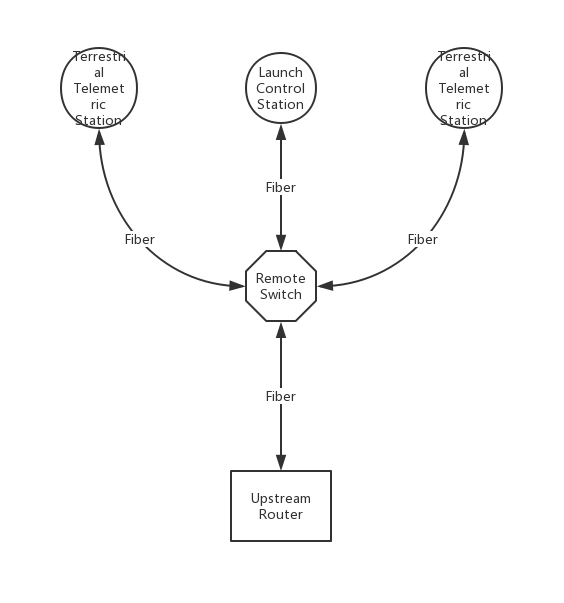
\includegraphics[width=0.58\textwidth]{img/ES00004_MCF.png}
 \caption{Block Diagram For Main Control Facility}	
\end{center}
\end{figure}
\newpage
\chapter{Launch Control Station (LCS)}
The Launch Control Station is majorly use to performs a launch sequence. It will take care all the need of the rocket and report the rocket status before launch. It also offer emergent cutoff. \\
It will have ability to perform any action the launch pad needed, which will be execute one processor inside the station. It will have ability to connect to the Main Control Facility.
\newpage
\chapter{Terrestrial Telemetric Station (TTS)}
The Terrestrial Telemetric Station performs basic analysis on the live telemetry data. This includes displaying a Range Safe/Range Live indication, vehicle orientation from sensor fusion, flight profile stages, and error monitoring.\\
The Terrestrial Telemetric Station is proform two jobs. The first job is monitering the vehicle status via the radio module. It will report the data it receive to the Main Control Facility connect to it. 
\newpage
\chapter{Ground Testing Station(GTS)}
The Ground Testing Station is majorly for the engine testing. It will help Main Control Facility to record and report testing engine thrust and thermo condition. It also will offer control on the rocket engine such as increase or cutoff fuel and oxidizer supply.
% End of document.
%**********************************************************************
\end{document}